\documentclass[16pt]{article}
\usepackage[utf8]{inputenc, lscape}
\usepackage[demo]{graphicx}
\usepackage[a4paper,bindingoffset=0.2in,%
            left=1.1in,right=0.85in,top=1in,bottom=1in,%
            footskip=.25in]{geometry}

\begin{document}

% this stuff is about to be presented to Alan on 09/(02-04)/19

% the scripts used:
% sp19_rm_22 for all monthly tables
% sp19_dailycimad_betas_7_49 for Figure 1.
% sp19_annually, semiannualy, quarterly_2.
% sp19_rm_21_5-10-17-30-49 for industries tables
% sp19_industry_partitions for short industry tables.

\newgeometry{left=1.5cm, right=1cm, top=3cm, bottom=1.5cm}

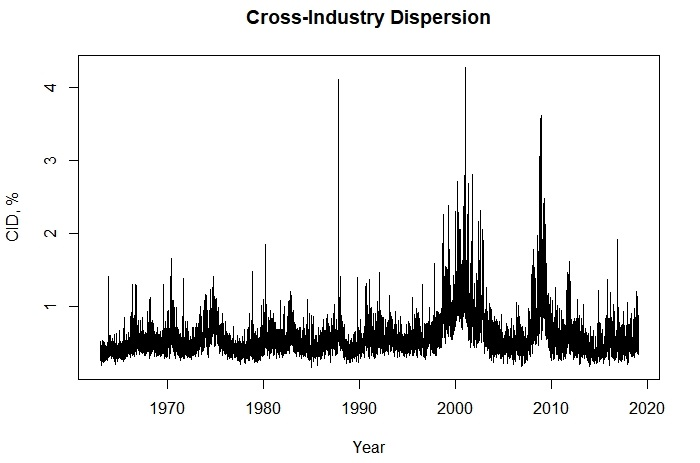
\includegraphics[width=1\textwidth]{ts_cid_00.jpeg}

\newpage

\textbf{Results with monthly returns:}

% Table created by stargazer v.5.2.2 by Marek Hlavac, Harvard University. E-mail: hlavac at fas.harvard.edu
% Date and time: Mon, Sep 02, 2019 - 9:55:18 AM
\begin{table}[!htbp] \centering 
  \caption{Characteristics of decile $\beta_{CID}$-sorted vw portfolios} 
  \label{} 
\begin{tabular}{@{\extracolsep{5pt}} cccccccccccc} 
\\[-1.8ex]\hline 
\hline \\[-1.8ex] 
 & D1 & D2 & D3 & D4 & D5 & D6 & D7 & D8 & D9 & D10 & LS \\ 
\hline \\[-1.8ex] 
RET & $1.17$ & $0.88$ & $0.86$ & $0.71$ & $0.63$ & $0.65$ & $0.65$ & $0.60$ & $0.52$ & $0.47$ & $$-$0.70$ \\ 
RET\_tstat & $4.80$ & $4.38$ & $4.56$ & $3.97$ & $3.73$ & $3.87$ & $3.69$ & $3.48$ & $2.79$ & $2.12$ & $$-$3.87$ \\ 
prebeta & $$-$1.55$ & $$-$0.86$ & $$-$0.51$ & $$-$0.26$ & $$-$0.05$ & $0.16$ & $0.38$ & $0.62$ & $0.96$ & $1.62$ & $3.16$ \\ 
postbeta & $$-$0.03$ & $0.12$ & $0.18$ & $0.23$ & $0.31$ & $0.32$ & $0.33$ & $0.41$ & $0.46$ & $0.58$ & $0.62$ \\ 
size & $7.11$ & $7.71$ & $8.13$ & $8.37$ & $8.60$ & $8.81$ & $8.96$ & $9.16$ & $9.15$ & $8.85$ & $1.74$ \\ 
bm & $6.05$ & $6.12$ & $6.13$ & $6.14$ & $6.14$ & $6.11$ & $6.11$ & $6.07$ & $6.01$ & $5.97$ & $$-$0.08$ \\ 
op & $0.15$ & $0.16$ & $0.17$ & $0.17$ & $0.17$ & $0.17$ & $0.17$ & $0.18$ & $0.18$ & $0.17$ & $0.02$ \\ 
inv & $0.29$ & $0.23$ & $0.18$ & $0.16$ & $0.14$ & $0.13$ & $0.13$ & $0.14$ & $0.14$ & $0.17$ & $$-$0.12$ \\ 
beta & $1.07$ & $0.96$ & $0.91$ & $0.88$ & $0.88$ & $0.89$ & $0.92$ & $0.98$ & $1.08$ & $1.31$ & $0.23$ \\ 
BAspr & $0.39$ & $0.32$ & $0.26$ & $0.24$ & $0.23$ & $0.21$ & $0.20$ & $0.19$ & $0.18$ & $0.18$ & $$-$0.21$ \\ 
mom122 & $0.24$ & $0.18$ & $0.15$ & $0.14$ & $0.12$ & $0.12$ & $0.11$ & $0.11$ & $0.11$ & $0.14$ & $$-$0.10$ \\ 
vol1m & $2.47$ & $2.02$ & $1.82$ & $1.72$ & $1.66$ & $1.61$ & $1.60$ & $1.63$ & $1.74$ & $2.03$ & $$-$0.44$ \\ 
vol12m & $2.63$ & $2.12$ & $1.90$ & $1.79$ & $1.72$ & $1.68$ & $1.67$ & $1.71$ & $1.83$ & $2.19$ & $$-$0.43$ \\ 
\hline \\[-1.8ex] 
\end{tabular} 
\end{table}


% Table created by stargazer v.5.2.2 by Marek Hlavac, Harvard University. E-mail: hlavac at fas.harvard.edu
% Date and time: Mon, Sep 02, 2019 - 9:56:17 AM
\begin{table}[!htbp] \centering 
  \caption{Returns of decile $\beta_{CID}$-sorted portfolios} 
  \label{} 
\begin{tabular}{@{\extracolsep{5pt}} cccccccccccc} 
\\[-1.8ex]\hline 
\hline \\[-1.8ex] 
 & D1 & D2 & D3 & D4 & D5 & D6 & D7 & D8 & D9 & D10 & LS \\ 
\hline \\[-1.8ex] 
Mean ew & $2.50$ & $1.79$ & $1.58$ & $1.41$ & $1.36$ & $1.32$ & $1.29$ & $1.26$ & $1.29$ & $1.61$ & $$-$0.89$ \\ 
T\_stat ew & $9.65$ & $8.70$ & $8.15$ & $7.73$ & $7.48$ & $7.26$ & $6.84$ & $6.52$ & $6.34$ & $6.45$ & $$-$5.72$ \\ 
Mean vw & $1.17$ & $0.88$ & $0.86$ & $0.71$ & $0.63$ & $0.65$ & $0.65$ & $0.60$ & $0.52$ & $0.47$ & $$-$0.70$ \\ 
T\_stat vw & $4.80$ & $4.38$ & $4.56$ & $3.97$ & $3.73$ & $3.87$ & $3.69$ & $3.48$ & $2.79$ & $2.12$ & $$-$3.87$ \\ 
\hline \\[-1.8ex] 
\end{tabular} 
\end{table}


% Table created by stargazer v.5.2.2 by Marek Hlavac, Harvard University. E-mail: hlavac at fas.harvard.edu
% Date and time: Mon, Sep 02, 2019 - 9:57:34 AM
\begin{table}[!htbp] \centering 
  \caption{Abnormal returns of decile $\beta_{CID}$-sorted vw portfolios} 
  \label{} 
\begin{tabular}{@{\extracolsep{5pt}} ccccccc} 
\\[-1.8ex]\hline 
\hline \\[-1.8ex] 
Statistic & Ret & Alpha CAPM & Alpha FF3 & Alpha Carhart & Alpha FF5 & Alpha FF5+UMD+STR \\ 
\hline \\[-1.8ex] 
Return & -0.70 & -0.67 & -0.75 & -0.55 & -0.80 & -0.50 \\ 
T-stat & [ -3.87] & [ -3.68] & [ -4.44] & [ -3.24] & [ -4.59] & [ -2.90] \\ 
\hline \\[-1.8ex] 
\end{tabular} 
\end{table} 



% Table created by stargazer v.5.2.2 by Marek Hlavac, Harvard University. E-mail: hlavac at fas.harvard.edu
% Date and time: Mon, Sep 02, 2019 - 9:59:41 AM
\begin{table}[!htbp] \centering 
  \caption{Factor loadings of decile $\beta_{CID}$-sorted vw portfolios} 
  \label{} 
\begin{tabular}{@{\extracolsep{5pt}} ccccccccccc} 
\\[-1.8ex]\hline 
\hline \\[-1.8ex] 
Ntile & Ret & Alpha & EMKT & HML & SMB & RMW & CMA & Mom & STR & adjR2 \\ 
\hline \\[-1.8ex] 
1 & 1.17 & 0.57 & 1.03 & -0.07 & 0.42 & -0.23 & -0.34 & 0.16 & 0.12 & 0.83 \\ 
 & [ 4.80] & [ 5.24] & [ 38.82] & [ -1.37] & [ 11.75] & [ -4.61] & [ -4.57] & [ 6.39] & [ 3.41] &  \\ 
2 & 0.88 & 0.22 & 0.97 & 0.05 & 0.23 & 0.07 & -0.15 & 0.12 & 0.10 & 0.84 \\ 
 & [ 4.38] & [ 2.46] & [ 45.09] & [ 1.18] & [ 7.84] & [ 1.63] & [ -2.43] & [ 5.67] & [ 3.48] &  \\ 
3 & 0.86 & 0.28 & 0.95 & 0.03 & 0.13 & -0.02 & -0.10 & 0.12 & 0.04 & 0.84 \\ 
 & [ 4.56] & [ 3.40] & [ 47.65] & [ 0.66] & [ 4.98] & [ -0.45] & [ -1.75] & [ 6.48] & [ 1.60] &  \\ 
4 & 0.71 & 0.07 & 0.96 & 0.03 & 0.08 & 0.14 & 0.05 & 0.08 & 0.07 & 0.86 \\ 
 & [ 3.97] & [ 0.92] & [ 54.98] & [ 1.00] & [ 3.56] & [ 4.13] & [ 1.03] & [ 4.67] & [ 2.99] &  \\ 
5 & 0.63 & 0.00 & 0.94 & 0.04 & 0.08 & 0.14 & 0.17 & 0.05 & 0.01 & 0.88 \\ 
 & [ 3.73] & [ -0.02] & [ 60.62] & [ 1.43] & [ 3.60] & [ 4.91] & [ 3.97] & [ 3.37] & [ 0.64] &  \\ 
6 & 0.65 & 0.07 & 0.92 & 0.02 & -0.01 & 0.13 & 0.10 & 0.02 & 0.06 & 0.88 \\ 
 & [ 3.87] & [ 1.20] & [ 60.34] & [ 0.70] & [ -0.27] & [ 4.62] & [ 2.33] & [ 1.38] & [ 3.11] &  \\ 
7 & 0.65 & 0.08 & 0.98 & 0.03 & -0.04 & 0.11 & 0.13 & -0.02 & 0.05 & 0.90 \\ 
 & [ 3.69] & [ 1.36] & [ 67.63] & [ 1.10] & [ -1.81] & [ 3.84] & [ 3.25] & [ -1.65] & [ 2.72] &  \\ 
8 & 0.60 & 0.03 & 1.01 & 0.12 & -0.08 & 0.18 & 0.12 & -0.04 & 0.00 & 0.91 \\ 
 & [ 3.48] & [ 0.47] & [ 74.54] & [ 4.69] & [ -4.30] & [ 7.16] & [ 3.14] & [ -2.98] & [ -0.24] &  \\ 
9 & 0.52 & 0.04 & 1.03 & 0.07 & -0.10 & 0.05 & 0.08 & -0.09 & -0.03 & 0.88 \\ 
 & [ 2.79] & [ 0.60] & [ 60.97] & [ 2.13] & [ -4.17] & [ 1.59] & [ 1.59] & [ -5.27] & [ -1.37] &  \\ 
10 & 0.47 & 0.07 & 1.16 & 0.14 & -0.04 & -0.12 & -0.11 & -0.13 & -0.13 & 0.83 \\ 
 & [ 2.12] & [ 0.71] & [ 47.98] & [ 3.07] & [ -1.15] & [ -2.71] & [ -1.64] & [ -5.54] & [ -3.96] &  \\ 
LS & -0.70 & -0.50 & 0.13 & 0.21 & -0.46 & 0.11 & 0.23 & -0.29 & -0.25 & 0.23 \\ 
 & [ -3.87] & [ -2.90] & [ 3.04] & [ 2.62] & [ -8.05] & [ 1.35] & [ 1.94] & [ -7.20] & [ -4.41] &  \\ 
\hline \\[-1.8ex] 
\end{tabular} 
\end{table}



% Table created by stargazer v.5.2.2 by Marek Hlavac, Harvard University. E-mail: hlavac at fas.harvard.edu
% Date and time: Mon, Sep 02, 2019 - 10:01:19 AM
\begin{table}[!htbp] \centering 
  \caption{Abnormal returns of 2x3 doublesorted portfolios on size and $\beta_{CID}$} 
  \label{} 
\begin{tabular}{@{\extracolsep{5pt}} ccccccc} 
\\[-1.8ex]\hline 
\hline \\[-1.8ex] 
Statistic & Ret & Alpha,CAPM & Alpha,FF3 & Alpha,Carhart & Alpha,FF5 & Alpha,FF5+UMD+STR \\ 
\hline \\[-1.8ex] 
Size L/S & 0.740 & 0.671 & 0.507 & 0.564 & 0.472 & 0.522 \\ 
 & [ 7.377] & [ 6.840] & [ 12.348] & [ 13.915] & [ 11.299] & [ 12.656] \\ 
CID L/S & 0.217 & 0.233 & 0.278 & 0.151 & 0.308 & 0.156 \\ 
 & [ 2.241] & [ 2.400] & [ 2.910] & [ 1.592] & [ 3.133] & [ 1.606] \\ 
\hline \\[-1.8ex] 
\end{tabular} 
\end{table}


% Table created by stargazer v.5.2.2 by Marek Hlavac, Harvard University. E-mail: hlavac at fas.harvard.edu
% Date and time: Mon, Sep 02, 2019 - 10:04:05 AM
\begin{table}[!htbp] \centering 
  \caption{Abnormal returns of 5x5 doublesorted portfolios on within-industry dispersion $\beta_{WID}$ and $\beta_{CID}$} 
  \label{} 
\begin{tabular}{@{\extracolsep{5pt}} ccccccc} 
\\[-1.8ex]\hline 
\hline \\[-1.8ex] 
Statistic & Ret & Alpha,CAPM & Alpha,FF3 & Alpha,Carhart & Alpha,FF5 & Alpha,FF5+UMD+STR \\ 
\hline \\[-1.8ex] 
L/S WID & 0.132 & 0.225 & 0.092 & -0.030 & -0.157 & -0.191 \\ 
& [ 0.888] & [ 1.459] & [ 0.607] & [ -0.195] & [ -1.077] & [ -1.275] \\ 
L/S CID & 0.381 & 0.342 & 0.436 & 0.384 & 0.590 & 0.429 \\ 
& [ 2.751] & [ 2.330] & [ 3.163] & [ 2.724] & [ 4.275] & [ 3.064] \\ 
\hline \\[-1.8ex] 
\end{tabular} 
\end{table}



% Table created by stargazer v.5.2.2 by Marek Hlavac, Harvard University. E-mail: hlavac at fas.harvard.edu
% Date and time: Mon, Sep 02, 2019 - 10:08:20 AM
\begin{table}[!htbp] \centering 
  \caption{Abnormal returns of 5x5 doublesorted portfolios on cross-sectional dispersion $\beta_{CSD}$ and $\beta_{CID}$} 
  \label{} 
\begin{tabular}{@{\extracolsep{5pt}} ccccccc} 
\\[-1.8ex]\hline 
\hline \\[-1.8ex] 
Statistic & Ret & Alpha,CAPM & Alpha,FF3 & Alpha,Carhart & Alpha,FF5 & Alpha,FF5+UMD+STR \\ 
\hline \\[-1.8ex] 
L/S CSD & -0.028 & 0.071 & -0.033 & -0.151 & -0.212 & -0.319 \\ 
& [ -0.200] & [ 0.493] & [ -0.236] & [ -1.057] & [ -1.522] & [ -2.243] \\ 
L/S CID & 0.324 & 0.283 & 0.304 & 0.262 & 0.430 & 0.315 \\ 
& [ 2.455] & [ 2.059] & [ 2.360] & [ 1.998] & [ 3.310] & [ 2.377] \\ 
\hline \\[-1.8ex] 
\end{tabular} 
\end{table}



% Table created by stargazer v.5.2.2 by Marek Hlavac, Harvard University. E-mail: hlavac at fas.harvard.edu
% Date and time: Mon, Sep 02, 2019 - 10:11:18 AM
\begin{table}[!htbp] \centering 
  \caption{Abnormal returns of 5x5 doublesorted portfolios on VIX and $\beta_{CID}$} 
  \label{} 
\begin{tabular}{@{\extracolsep{5pt}} ccccccc} 
\\[-1.8ex]\hline 
\hline \\[-1.8ex] 
Statistic & Ret & Alpha,CAPM & Alpha,FF3 & Alpha,Carhart & Alpha,FF5 & Alpha,FF5+UMD+STR \\ 
\hline \\[-1.8ex] 
L/S VIX & 0.248 & -0.126 & -0.088 & 0.052 & 0.192 & 0.275 \\ 
& [ 1.080] & [ -0.681] & [ -0.495] & [ 0.299] & [ 1.097] & [ 1.606] \\ 
L/S CID & 0.238 & 0.237 & 0.384 & 0.217 & 0.304 & 0.155 \\ 
& [ 1.204] & [ 1.186] & [ 2.123] & [ 1.242] & [ 1.636] & [ 0.869] \\ 
\hline \\[-1.8ex] 
\end{tabular} 
\end{table}



% Table created by stargazer v.5.2.2 by Marek Hlavac, Harvard University. E-mail: hlavac at fas.harvard.edu
% Date and time: Mon, Sep 02, 2019 - 10:13:03 AM
\begin{table}[!htbp] \centering 
  \caption{Abnormal returns of 5x5 doublesorted portfolios on CIV (Kelly16) and $\beta_{CID}$} 
  \label{} 
\begin{tabular}{@{\extracolsep{5pt}} ccccccc} 
\\[-1.8ex]\hline 
\hline \\[-1.8ex] 
Statistic & Ret & Alpha,CAPM & Alpha,FF3 & Alpha,Carhart & Alpha,FF5 & Alpha,FF5+UMD+STR \\ 
\hline \\[-1.8ex] 
L/S CIV & 0.330 & 0.267 & 0.165 & 0.211 & 0.079 & 0.127 \\ 
& [ 2.754] & [ 2.252] & [ 1.406] & [ 1.764] & [ 0.660] & [ 1.042] \\ 
L/S CID & 0.370 & 0.392 & 0.424 & 0.261 & 0.443 & 0.233 \\ 
& [ 3.058] & [ 3.224] & [ 3.644] & [ 2.273] & [ 3.703] & [ 1.989] \\ 
\hline \\[-1.8ex] 
\end{tabular} 
\end{table}



% Table created by stargazer v.5.2.2 by Marek Hlavac, Harvard University. E-mail: hlavac at fas.harvard.edu
% Date and time: Mon, Sep 02, 2019 - 10:14:30 AM
\begin{table}[!htbp] \centering 
  \caption{Abnormal returns of 5x5 double-sorted portfolios on macroeconomic uncertainty (Ludvigson15) and $\beta_{CID}$} 
  \label{} 
\begin{tabular}{@{\extracolsep{5pt}} ccccccc} 
\\[-1.8ex]\hline 
\hline \\[-1.8ex] 
Statistic & Ret & Alpha,CAPM & Alpha,FF3 & Alpha,Carhart & Alpha,FF5 & Alpha,FF5+UMD+STR \\ 
\hline \\[-1.8ex] 
L/S MU & 0.047 & -0.069 & -0.027 & 0.075 & 0.187 & 0.193 \\ 
& [ 0.330] & [ -0.497] & [ -0.202] & [ 0.555] & [ 1.426] & [ 1.444] \\ 
L/S CID & 0.489 & 0.490 & 0.526 & 0.349 & 0.542 & 0.323 \\ 
& [ 3.757] & [ 3.741] & [ 4.192] & [ 2.820] & [ 4.201] & [ 2.547] \\ 
\hline \\[-1.8ex] 
\end{tabular} 
\end{table}


% Table created by stargazer v.5.2.2 by Marek Hlavac, Harvard University. E-mail: hlavac at fas.harvard.edu
% Date and time: Mon, Sep 02, 2019 - 10:16:03 AM
\begin{table}[!htbp] \centering 
  \caption{Abnormal returns of 5x5 double-sorted portfolios on financial uncertainty (Ludvigson15) and $\beta_{CID}$} 
  \label{} 
\begin{tabular}{@{\extracolsep{5pt}} ccccccc} 
\\[-1.8ex]\hline 
\hline \\[-1.8ex] 
Statistic & Ret & Alpha,CAPM & Alpha,FF3 & Alpha,Carhart & Alpha,FF5 & Alpha,FF5+UMD+STR \\ 
\hline \\[-1.8ex] 
L/S FU & 0.252 & 0.151 & 0.009 & -0.038 & -0.102 & -0.071 \\ 
& [ 1.850] & [ 1.144] & [ 0.067] & [ -0.294] & [ -0.788] & [ -0.532] \\ 
L/S CID & 0.391 & 0.396 & 0.438 & 0.315 & 0.445 & 0.282 \\ 
& [ 3.250] & [ 3.275] & [ 3.749] & [ 2.686] & [ 3.696] & [ 2.334] \\ 
\hline \\[-1.8ex] 
\end{tabular} 
\end{table}



% Table created by stargazer v.5.2.2 by Marek Hlavac, Harvard University. E-mail: hlavac at fas.harvard.edu
% Date and time: Mon, Sep 02, 2019 - 10:17:25 AM
\begin{table}[!htbp] \centering 
  \caption{Abnormal returns of 5x5 double-sorted portfolios on market volatility over 24 months and $\beta_{CID}$} 
  \label{} 
\begin{tabular}{@{\extracolsep{5pt}} ccccccc} 
\\[-1.8ex]\hline 
\hline \\[-1.8ex] 
Statistic & Ret & Alpha,CAPM & Alpha,FF3 & Alpha,Carhart & Alpha,FF5 & Alpha,FF5+UMD+STR \\ 
\hline \\[-1.8ex] 
L/S VOL & 0.305 & 0.179 & 0.253 & 0.286 & 0.487 & 0.474 \\ 
& [ 2.218] & [ 1.362] & [ 1.965] & [ 2.179] & [ 3.850] & [ 3.637] \\ 
L/S CID & 0.402 & 0.420 & 0.449 & 0.319 & 0.482 & 0.297 \\ 
& [ 3.314] & [ 3.448] & [ 3.836] & [ 2.721] & [ 4.002] & [ 2.475] \\ 
\hline \\[-1.8ex] 
\end{tabular} 
\end{table}






\newpage

\textbf{Results with quarterly returns:}

% Table created by stargazer v.5.2.2 by Marek Hlavac, Harvard University. E-mail: hlavac at fas.harvard.edu
% Date and time: Mon, Sep 02, 2019 - 10:52:22 AM
\begin{table}[!htbp] \centering 
  \caption{Quarterly returns of decile $\beta_{CID}$-sorted portfolios} 
  \label{} 
\begin{tabular}{@{\extracolsep{5pt}} cccccccccccc} 
\\[-1.8ex]\hline 
\hline \\[-1.8ex] 
 & D1 & D2 & D3 & D4 & D5 & D6 & D7 & D8 & D9 & D10 & LS \\ 
\hline \\[-1.8ex] 
Mean ew & $4.26$ & $3.73$ & $3.54$ & $3.11$ & $3.18$ & $3.03$ & $2.90$ & $2.71$ & $2.74$ & $3.01$ & $$-$1.25$ \\ 
T\_stat ew & $5.02$ & $5.35$ & $5.32$ & $4.90$ & $5.07$ & $4.82$ & $4.45$ & $4.09$ & $3.96$ & $3.65$ & $$-$2.72$ \\ 
Mean vw & $2.61$ & $2.40$ & $2.20$ & $1.83$ & $1.85$ & $1.76$ & $1.79$ & $1.52$ & $1.67$ & $1.32$ & $$-$1.29$ \\ 
T\_stat vw & $3.25$ & $3.57$ & $3.49$ & $3.12$ & $3.33$ & $3.40$ & $3.17$ & $2.65$ & $2.87$ & $1.83$ & $$-$2.30$ \\ 
\hline \\[-1.8ex] 
\end{tabular} 
\end{table} 

\vspace{-0.32cm}

% Table created by stargazer v.5.2.2 by Marek Hlavac, Harvard University. E-mail: hlavac at fas.harvard.edu
% Date and time: Mon, Sep 02, 2019 - 10:52:42 AM
\begin{table}[!htbp] \centering 
  \caption{Abnormal quarterly returns of decile $\beta_{CID}$-sorted portfolios} 
  \label{} 
\begin{tabular}{@{\extracolsep{5pt}} ccccccc} 
\\[-1.8ex]\hline 
\hline \\[-1.8ex] 
Statistic & Ret & Alpha CAPM & Alpha FF3 & Alpha Carhart & Alpha FF5 & Alpha FF5+UMD+STR \\  
\hline \\[-1.8ex] 
Return & -1.29 & -1.10 & -1.60 & -0.89 & -2.07 & -1.16 \\ 
 & [ -2.30] & [ -1.95] & [ -2.91] & [ -1.56] & [ -3.63] & [ -1.90] \\ 
\hline \\[-1.8ex] 
\end{tabular} 
\end{table}



\textbf{Results with semiannually returns:}

% Table created by stargazer v.5.2.2 by Marek Hlavac, Harvard University. E-mail: hlavac at fas.harvard.edu
% Date and time: Mon, Sep 02, 2019 - 4:14:41 PM
\begin{table}[!htbp] \centering 
  \caption{Semiannually returns of decile $\beta_{CID}$-sorted portfolios} 
  \label{} 
\begin{tabular}{@{\extracolsep{5pt}} cccccccccccc} 
\\[-1.8ex]\hline 
\hline \\[-1.8ex] 
 & D1 & D2 & D3 & D4 & D5 & D6 & D7 & D8 & D9 & D10 & LS \\ 
\hline \\[-1.8ex] 
Mean ew & $6.68$ & $6.50$ & $6.00$ & $5.28$ & $5.47$ & $5.43$ & $4.90$ & $4.80$ & $4.54$ & $4.57$ & $$-$2.11$ \\ 
T\_stat ew & $4.01$ & $4.43$ & $4.32$ & $4.11$ & $4.32$ & $4.17$ & $3.88$ & $3.68$ & $3.35$ & $2.96$ & $$-$2.32$ \\ 
Mean vw & $4.69$ & $4.62$ & $4.14$ & $3.58$ & $3.78$ & $3.28$ & $2.98$ & $3.25$ & $3.15$ & $2.45$ & $$-$2.24$ \\ 
T\_stat vw & $2.87$ & $3.46$ & $3.21$ & $3.00$ & $3.48$ & $3.15$ & $2.90$ & $2.82$ & $2.78$ & $1.82$ & $$-$2.02$ \\ 
\hline \\[-1.8ex] 
\end{tabular} 
\end{table}

\vspace{-0.32cm}

% Table created by stargazer v.5.2.2 by Marek Hlavac, Harvard University. E-mail: hlavac at fas.harvard.edu
% Date and time: Mon, Sep 02, 2019 - 4:14:54 PM
\begin{table}[!htbp] \centering 
  \caption{Abnormal semiannually returns of decile $\beta_{CID}$-sorted portfolios} 
  \label{} 
\begin{tabular}{@{\extracolsep{5pt}} ccccccc} 
\\[-1.8ex]\hline 
\hline \\[-1.8ex] 
Statistic & Ret & Alpha CAPM & Alpha FF3 & Alpha Carhart & Alpha FF5 & Alpha FF5+UMD+STR \\ 
\hline \\[-1.8ex] 
Return & -2.24 & -1.70 & -2.14 & -1.35 & -3.46 & -2.44 \\ 
 & [ -2.02] & [ -1.50] & [ -1.87] & [ -1.07] & [ -2.93] & [ -1.78] \\ 
\hline \\[-1.8ex] 
\end{tabular} 
\end{table}



\textbf{Results with annual returns:}

% Table created by stargazer v.5.2.2 by Marek Hlavac, Harvard University. E-mail: hlavac at fas.harvard.edu
% Date and time: Mon, Sep 02, 2019 - 4:25:09 PM
\begin{table}[!htbp] \centering 
  \caption{Annual returns of decile $\beta_{CID}$-sorted portfolios} 
  \label{} 
\begin{tabular}{@{\extracolsep{5pt}} cccccccccccc} 
\\[-1.8ex]\hline 
\hline \\[-1.8ex] 
 & D1 & D2 & D3 & D4 & D5 & D6 & D7 & D8 & D9 & D10 & LS \\ 
\hline \\[-1.8ex] 
Mean ew & $24.13$ & $18.38$ & $15.52$ & $13.91$ & $13.23$ & $13.63$ & $12.93$ & $13.38$ & $13.13$ & $16.38$ & $$-$7.75$ \\ 
T\_stat ew & $5.68$ & $5.08$ & $5.17$ & $5.00$ & $5.03$ & $5.09$ & $5.04$ & $4.92$ & $4.62$ & $4.86$ & $$-$3.62$ \\ 
Mean vw & $18.14$ & $13.95$ & $12.95$ & $10.91$ & $9.69$ & $9.87$ & $9.71$ & $9.90$ & $10.01$ & $11.08$ & $$-$7.06$ \\ 
T\_stat vw & $5.03$ & $4.68$ & $4.47$ & $4.24$ & $4.26$ & $4.43$ & $4.77$ & $4.11$ & $4.08$ & $3.89$ & $$-$3.01$ \\ 
\hline \\[-1.8ex] 
\end{tabular} 
\end{table}

\vspace{-0.32cm}

% Table created by stargazer v.5.2.2 by Marek Hlavac, Harvard University. E-mail: hlavac at fas.harvard.edu
% Date and time: Mon, Sep 02, 2019 - 4:25:25 PM
\begin{table}[!htbp] \centering 
  \caption{Abnormal annual returns of decile $\beta_{CID}$-sorted portfolios} 
  \label{} 
\begin{tabular}{@{\extracolsep{5pt}} ccccccc} 
\\[-1.8ex]\hline 
\hline \\[-1.8ex] 
Statistic & Ret & Alpha CAPM & Alpha FF3 & Alpha Carhart & Alpha FF5 & Alpha FF5+UMD+STR \\ 
\hline \\[-1.8ex] 
Return & -7.06 & -5.50 & -5.20 & -1.97 & -8.46 & -5.95 \\ 
 & [ -3.01] & [ -2.24] & [ -2.15] & [ -0.67] & [ -3.03] & [ -1.63] \\ 
\hline \\[-1.8ex] 
\end{tabular} 
\end{table} 


\newpage

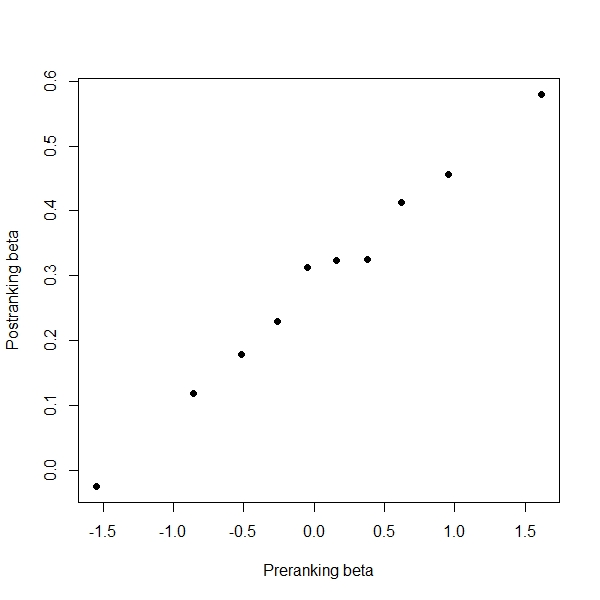
\includegraphics[width=1\textwidth]{Postranking.jpeg}
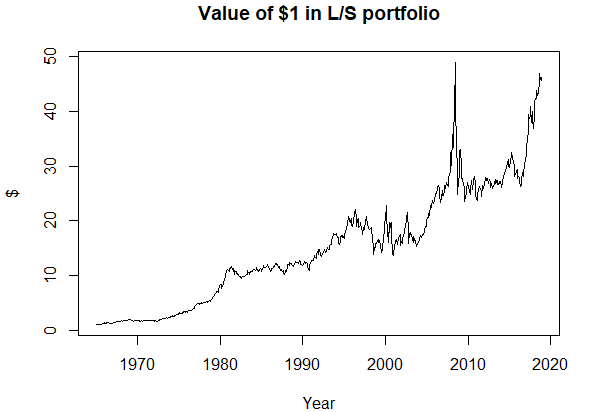
\includegraphics[width=1\textwidth]{performance.png}
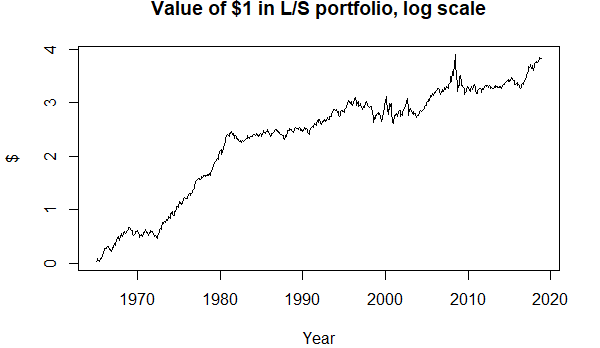
\includegraphics[width=1\textwidth]{performance,log.png}
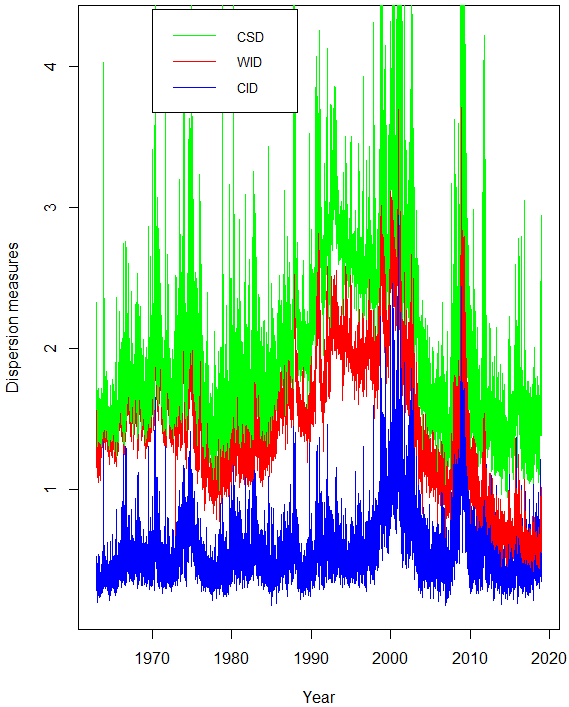
\includegraphics[width=1\textwidth]{fig1.png}
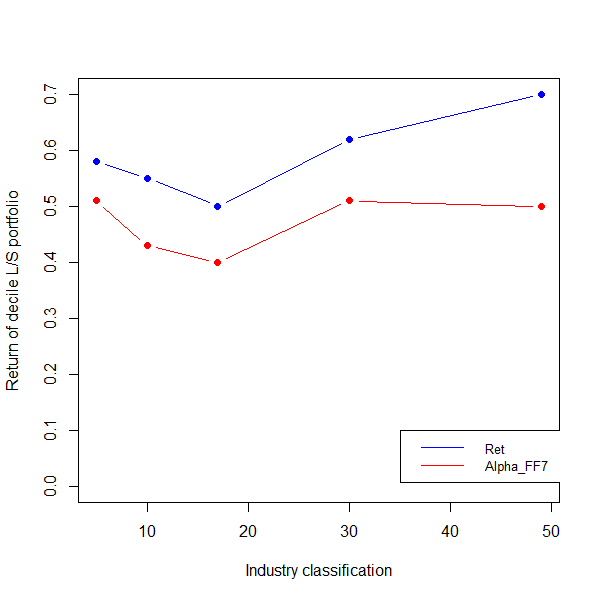
\includegraphics[width=1\textwidth]{alphas_inds.png}
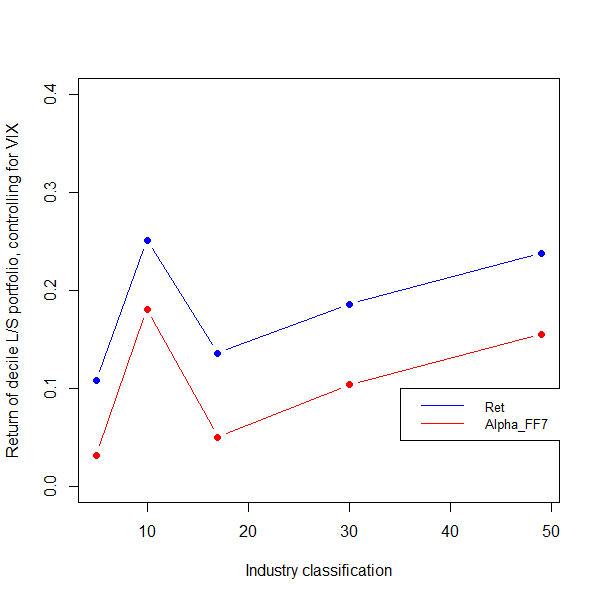
\includegraphics[width=1\textwidth]{alphas_vix_inds.png}
\newpage


\textbf{Results with monthly returns and different Fama-French industry partitions:}
\textbf{30 industries:}

% Table created by stargazer v.5.2.2 by Marek Hlavac, Harvard University. E-mail: hlavac at fas.harvard.edu
% Date and time: Mon, Sep 02, 2019 - 11:11:31 AM
\begin{table}[!htbp] \centering 
  \caption{Returns of monthly $\beta_{CID}$-sorted portfolios} 
  \label{} 
\begin{tabular}{@{\extracolsep{5pt}} cccccccccccc} 
\\[-1.8ex]\hline 
\hline \\[-1.8ex] 
 & D1 & D2 & D3 & D4 & D5 & D6 & D7 & D8 & D9 & D10 & LS \\ 
\hline \\[-1.8ex] 
Mean & $2.47$ & $1.74$ & $1.56$ & $1.40$ & $1.37$ & $1.34$ & $1.24$ & $1.23$ & $1.34$ & $1.61$ & $$-$0.86$ \\ 
T\_stat & $9.57$ & $8.46$ & $8.10$ & $7.56$ & $7.61$ & $7.37$ & $6.72$ & $6.32$ & $6.51$ & $6.56$ & $$-$5.52$ \\ 
Mean1 & $1.13$ & $0.91$ & $0.74$ & $0.77$ & $0.60$ & $0.69$ & $0.58$ & $0.58$ & $0.54$ & $0.51$ & $$-$0.62$ \\ 
T\_stat1 & $4.55$ & $4.42$ & $4.05$ & $4.38$ & $3.48$ & $4.13$ & $3.47$ & $3.37$ & $2.87$ & $2.30$ & $$-$3.35$ \\ 
\hline \\[-1.8ex] 
\end{tabular} 
\end{table}

% Table created by stargazer v.5.2.2 by Marek Hlavac, Harvard University. E-mail: hlavac at fas.harvard.edu
% Date and time: Mon, Sep 02, 2019 - 11:11:50 AM
\begin{table}[!htbp] \centering 
  \caption{Abnormal returns of monthly $\beta_{CID}$-sorted vw portfolios} 
  \label{} 
\begin{tabular}{@{\extracolsep{5pt}} ccccccc} 
\\[-1.8ex]\hline 
\hline \\[-1.8ex] 
Ntile & Ret & Alpha & Alpha.1 & Alpha.2 & Alpha.3 & Alpha.4 \\ 
\hline \\[-1.8ex] 
LS & -0.62 & -0.58 & -0.69 & -0.54 & -0.79 & -0.51 \\ 
 & [ -3.35] & [ -3.11] & [ -3.89] & [ -3.02] & [ -4.37] & [ -2.85] \\ 
\hline \\[-1.8ex] 
\end{tabular} 
\end{table}

% Table created by stargazer v.5.2.2 by Marek Hlavac, Harvard University. E-mail: hlavac at fas.harvard.edu
% Date and time: Mon, Sep 02, 2019 - 11:14:27 AM
\begin{table}[!htbp] \centering 
  \caption{Abnormal returns of 5x5 doublesorted portfolios on cross-sectional dispersion $\beta_{CSD}$ and $\beta_{CID}$} 
  \label{} 
\begin{tabular}{@{\extracolsep{5pt}} ccccccc} 
\\[-1.8ex]\hline 
\hline \\[-1.8ex] 
Statistic & Ret & Alpha,CAPM & Alpha,FF3 & Alpha,Carhart & Alpha,FF5 & Alpha,FF5+UMD+STR \\ 
\hline \\[-1.8ex] 
26 & 0.073 & 0.181 & 0.130 & -0.011 & -0.091 & -0.221 \\ 
beta\_csmad & [ 0.521] & [ 1.293] & [ 0.933] & [ -0.077] & [ -0.670] & [ -1.613] \\ 
LS & 0.347 & 0.295 & 0.304 & 0.286 & 0.441 & 0.350 \\ 
CID & [ 2.626] & [ 2.176] & [ 2.414] & [ 2.228] & [ 3.469] & [ 2.699] \\ 
\hline \\[-1.8ex] 
\end{tabular} 
\end{table}


% Table created by stargazer v.5.2.2 by Marek Hlavac, Harvard University. E-mail: hlavac at fas.harvard.edu
% Date and time: Mon, Sep 02, 2019 - 11:14:50 AM
\begin{table}[!htbp] \centering 
  \caption{Abnormal returns of 5x5 doublesorted portfolios on cross-sectional dispersion $\beta_{VIX}$ and $\beta_{CID}$} 
  \label{} 
\begin{tabular}{@{\extracolsep{5pt}} ccccccc} 
\\[-1.8ex]\hline 
\hline \\[-1.8ex] 
Statistic & Ret & Alpha,CAPM & Alpha,FF3 & Alpha,Carhart & Alpha,FF5 & Alpha,FF5+UMD+STR \\ 
\hline \\[-1.8ex] 
26 & 0.228 & -0.157 & -0.120 & 0.037 & 0.150 & 0.247 \\ 
beta\_vix & [ 0.987] & [ -0.856] & [ -0.678] & [ 0.213] & [ 0.852] & [ 1.443] \\ 
LS & 0.186 & 0.152 & 0.296 & 0.180 & 0.216 & 0.104 \\ 
CID & [ 0.952] & [ 0.770] & [ 1.649] & [ 1.010] & [ 1.182] & [ 0.580] \\ 
\hline \\[-1.8ex] 
\end{tabular} 
\end{table}

% Table created by stargazer v.5.2.2 by Marek Hlavac, Harvard University. E-mail: hlavac at fas.harvard.edu
% Date and time: Mon, Sep 02, 2019 - 11:15:20 AM
\begin{table}[!htbp] \centering 
  \caption{Abnormal returns of 5x5 doublesorted portfolios on cross-sectional dispersion $\beta_{CIV}$ and $\beta_{CID}$} 
  \label{} 
\begin{tabular}{@{\extracolsep{5pt}} ccccccc} 
\\[-1.8ex]\hline 
\hline \\[-1.8ex] 
Statistic & Ret & Alpha,CAPM & Alpha,FF3 & Alpha,Carhart & Alpha,FF5 & Alpha,FF5+UMD+STR \\ 
\hline \\[-1.8ex] 
26 & 0.359 & 0.300 & 0.195 & 0.233 & 0.119 & 0.153 \\ 
beta\_civ & [ 2.987] & [ 2.514] & [ 1.656] & [ 1.941] & [ 0.991] & [ 1.241] \\ 
LS & 0.334 & 0.343 & 0.380 & 0.269 & 0.432 & 0.270 \\ 
CID & [ 2.829] & [ 2.889] & [ 3.377] & [ 2.379] & [ 3.748] & [ 2.338] \\ 
\hline \\[-1.8ex] 
\end{tabular} 
\end{table}

\vspace{-0.32cm}

% Table created by stargazer v.5.2.2 by Marek Hlavac, Harvard University. E-mail: hlavac at fas.harvard.edu
% Date and time: Mon, Sep 02, 2019 - 11:15:35 AM
\begin{table}[!htbp] \centering 
  \caption{Abnormal returns of 5x5 doublesorted portfolios on cross-sectional dispersion $\beta_{VOL}$ and $\beta_{CID}$} 
  \label{} 
\begin{tabular}{@{\extracolsep{5pt}} ccccccc} 
\\[-1.8ex]\hline 
\hline \\[-1.8ex] 
Statistic & Ret & Alpha,CAPM & Alpha,FF3 & Alpha,Carhart & Alpha,FF5 & Alpha,FF5+UMD+STR \\ 
\hline \\[-1.8ex] 
26 & 0.335 & 0.209 & 0.282 & 0.316 & 0.522 & 0.506 \\ 
beta\_roll\_sd24 & [ 2.414] & [ 1.573] & [ 2.162] & [ 2.376] & [ 4.066] & [ 3.830] \\ 
LS & 0.338 & 0.351 & 0.385 & 0.291 & 0.445 & 0.284 \\ 
CID & [ 2.784] & [ 2.876] & [ 3.272] & [ 2.451] & [ 3.691] & [ 2.344] \\ 
\hline \\[-1.8ex] 
\end{tabular} 
\end{table}


\newpage

\textbf{Results with monthly returns and different Fama-French industry partitions:}
\textbf{17 industries:}

% Table created by stargazer v.5.2.2 by Marek Hlavac, Harvard University. E-mail: hlavac at fas.harvard.edu
% Date and time: Mon, Sep 02, 2019 - 11:21:37 AM
\begin{table}[!htbp] \centering 
  \caption{} 
  \label{} 
\begin{tabular}{@{\extracolsep{5pt}} cccccccccccc} 
\\[-1.8ex]\hline 
\hline \\[-1.8ex] 
 & D1 & D2 & D3 & D4 & D5 & D6 & D7 & D8 & D9 & D10 & LS \\ 
\hline \\[-1.8ex] 
Mean & $2.48$ & $1.75$ & $1.51$ & $1.39$ & $1.35$ & $1.30$ & $1.26$ & $1.25$ & $1.35$ & $1.68$ & $$-$0.79$ \\ 
T\_stat & $9.71$ & $8.64$ & $7.98$ & $7.58$ & $7.44$ & $7.14$ & $6.77$ & $6.44$ & $6.45$ & $6.72$ & $$-$5.33$ \\ 
Mean1 & $1.04$ & $0.90$ & $0.75$ & $0.75$ & $0.67$ & $0.63$ & $0.50$ & $0.64$ & $0.54$ & $0.54$ & $$-$0.50$ \\ 
T\_stat1 & $4.29$ & $4.52$ & $4.10$ & $4.27$ & $4.05$ & $3.75$ & $2.95$ & $3.65$ & $2.91$ & $2.43$ & $$-$2.78$ \\ 
\hline \\[-1.8ex] 
\end{tabular} 
\end{table} 

% Table created by stargazer v.5.2.2 by Marek Hlavac, Harvard University. E-mail: hlavac at fas.harvard.edu
% Date and time: Mon, Sep 02, 2019 - 11:21:51 AM
\begin{table}[!htbp] \centering 
  \caption{} 
  \label{} 
\begin{tabular}{@{\extracolsep{5pt}} ccccccc} 
\\[-1.8ex]\hline 
\hline \\[-1.8ex] 
Ntile & Ret & Alpha & Alpha.1 & Alpha.2 & Alpha.3 & Alpha.4 \\ 
\hline \\[-1.8ex] 
LS & -0.50 & -0.47 & -0.55 & -0.42 & -0.65 & -0.40 \\ 
 & [ -2.78] & [ -2.59] & [ -3.13] & [ -2.37] & [ -3.61] & [ -2.22] \\ 
\hline \\[-1.8ex] 
\end{tabular} 
\end{table}

% Table created by stargazer v.5.2.2 by Marek Hlavac, Harvard University. E-mail: hlavac at fas.harvard.edu
% Date and time: Mon, Sep 02, 2019 - 11:22:10 AM
\begin{table}[!htbp] \centering 
  \caption{} 
  \label{} 
\begin{tabular}{@{\extracolsep{5pt}} ccccccc} 
\\[-1.8ex]\hline 
\hline \\[-1.8ex] 
Statistic & Ret & Alpha,CAPM & Alpha,FF3 & Alpha,Carhart & Alpha,FF5 & Alpha,FF5+UMD+STR \\ 
\hline \\[-1.8ex] 
26 & 0.225 & 0.347 & 0.301 & 0.153 & 0.074 & -0.044 \\ 
beta\_csmad & [ 1.608] & [ 2.527] & [ 2.200] & [ 1.121] & [ 0.559] & [ -0.325] \\ 
LS & 0.204 & 0.161 & 0.144 & 0.158 & 0.268 & 0.190 \\ 
CID & [ 1.682] & [ 1.301] & [ 1.240] & [ 1.330] & [ 2.267] & [ 1.584] \\ 
\hline \\[-1.8ex] 
\end{tabular} 
\end{table}

% Table created by stargazer v.5.2.2 by Marek Hlavac, Harvard University. E-mail: hlavac at fas.harvard.edu
% Date and time: Mon, Sep 02, 2019 - 11:22:27 AM
\begin{table}[!htbp] \centering 
  \caption{} 
  \label{} 
\begin{tabular}{@{\extracolsep{5pt}} ccccccc} 
\\[-1.8ex]\hline 
\hline \\[-1.8ex] 
Statistic & Ret & Alpha,CAPM & Alpha,FF3 & Alpha,Carhart & Alpha,FF5 & Alpha,FF5+UMD+STR \\ 
\hline \\[-1.8ex] 
26 & 0.186 & -0.213 & -0.169 & -0.007 & 0.116 & 0.215 \\ 
beta\_vix & [ 0.791] & [ -1.157] & [ -0.957] & [ -0.044] & [ 0.670] & [ 1.281] \\ 
LS & 0.136 & 0.123 & 0.257 & 0.141 & 0.157 & 0.050 \\ 
CID & [ 0.693] & [ 0.619] & [ 1.412] & [ 0.781] & [ 0.850] & [ 0.272] \\ 
\hline \\[-1.8ex] 
\end{tabular} 
\end{table}

% Table created by stargazer v.5.2.2 by Marek Hlavac, Harvard University. E-mail: hlavac at fas.harvard.edu
% Date and time: Mon, Sep 02, 2019 - 11:22:43 AM
\begin{table}[!htbp] \centering 
  \caption{} 
  \label{} 
\begin{tabular}{@{\extracolsep{5pt}} ccccccc} 
\\[-1.8ex]\hline 
\hline \\[-1.8ex] 
Statistic & Ret & Alpha,CAPM & Alpha,FF3 & Alpha,Carhart & Alpha,FF5 & Alpha,FF5+UMD+STR \\ 
\hline \\[-1.8ex] 
26 & 0.351 & 0.286 & 0.184 & 0.217 & 0.102 & 0.144 \\ 
beta\_civ & [ 2.896] & [ 2.384] & [ 1.553] & [ 1.793] & [ 0.842] & [ 1.159] \\ 
LS & 0.323 & 0.345 & 0.364 & 0.262 & 0.398 & 0.233 \\ 
CID & [ 2.705] & [ 2.875] & [ 3.141] & [ 2.239] & [ 3.339] & [ 1.952] \\ 
\hline \\[-1.8ex] 
\end{tabular} 
\end{table}

% Table created by stargazer v.5.2.2 by Marek Hlavac, Harvard University. E-mail: hlavac at fas.harvard.edu
% Date and time: Mon, Sep 02, 2019 - 11:23:01 AM
\begin{table}[!htbp] \centering 
  \caption{} 
  \label{} 
\begin{tabular}{@{\extracolsep{5pt}} ccccccc} 
\\[-1.8ex]\hline 
\hline \\[-1.8ex] 
Statistic & Ret & Alpha,CAPM & Alpha,FF3 & Alpha,Carhart & Alpha,FF5 & Alpha,FF5+UMD+STR \\ 
\hline \\[-1.8ex] 
26 & 0.337 & 0.206 & 0.281 & 0.317 & 0.528 & 0.514 \\ 
beta\_roll\_sd24 & [ 2.392] & [ 1.533] & [ 2.140] & [ 2.370] & [ 4.106] & [ 3.880] \\ 
LS & 0.288 & 0.311 & 0.327 & 0.237 & 0.373 & 0.213 \\ 
CID & [ 2.380] & [ 2.553] & [ 2.753] & [ 1.969] & [ 3.059] & [ 1.740] \\ 
\hline \\[-1.8ex] 
\end{tabular} 
\end{table}



\newpage

\textbf{Results with monthly returns and different Fama-French industry partitions:}
\textbf{10 industries:}

% Table created by stargazer v.5.2.2 by Marek Hlavac, Harvard University. E-mail: hlavac at fas.harvard.edu
% Date and time: Mon, Sep 02, 2019 - 11:27:55 AM
\begin{table}[!htbp] \centering 
  \caption{} 
  \label{} 
\begin{tabular}{@{\extracolsep{5pt}} cccccccccccc} 
\\[-1.8ex]\hline 
\hline \\[-1.8ex] 
 & D1 & D2 & D3 & D4 & D5 & D6 & D7 & D8 & D9 & D10 & LS \\ 
\hline \\[-1.8ex] 
Mean & $2.41$ & $1.72$ & $1.52$ & $1.44$ & $1.32$ & $1.28$ & $1.34$ & $1.23$ & $1.33$ & $1.72$ & $$-$0.69$ \\ 
T\_stat & $9.25$ & $8.40$ & $8.10$ & $7.86$ & $7.28$ & $7.09$ & $7.16$ & $6.38$ & $6.41$ & $6.87$ & $$-$4.55$ \\ 
Mean1 & $1.02$ & $0.89$ & $0.71$ & $0.76$ & $0.66$ & $0.63$ & $0.63$ & $0.54$ & $0.52$ & $0.49$ & $$-$0.55$ \\ 
T\_stat1 & $4.15$ & $4.47$ & $3.96$ & $4.39$ & $3.87$ & $3.71$ & $3.74$ & $3.07$ & $2.81$ & $2.18$ & $$-$3.03$ \\ 
\hline \\[-1.8ex] 
\end{tabular} 
\end{table} 

% Table created by stargazer v.5.2.2 by Marek Hlavac, Harvard University. E-mail: hlavac at fas.harvard.edu
% Date and time: Mon, Sep 02, 2019 - 11:28:18 AM
\begin{table}[!htbp] \centering 
  \caption{} 
  \label{} 
\begin{tabular}{@{\extracolsep{5pt}} ccccccc} 
\\[-1.8ex]\hline 
\hline \\[-1.8ex] 
Ntile & Ret & Alpha & Alpha.1 & Alpha.2 & Alpha.3 & Alpha.4 \\ 
\hline \\[-1.8ex] 
LS & -0.55 & -0.53 & -0.62 & -0.48 & -0.71 & -0.43 \\ 
 & [ -3.05] & [ -2.86] & [ -3.58] & [ -2.74] & [ -4.03] & [ -2.44] \\ 
\hline \\[-1.8ex] 
\end{tabular} 
\end{table}

% Table created by stargazer v.5.2.2 by Marek Hlavac, Harvard University. E-mail: hlavac at fas.harvard.edu
% Date and time: Mon, Sep 02, 2019 - 11:28:43 AM
\begin{table}[!htbp] \centering 
  \caption{} 
  \label{} 
\begin{tabular}{@{\extracolsep{5pt}} ccccccc} 
\\[-1.8ex]\hline 
\hline \\[-1.8ex] 
Statistic & Ret & Alpha,CAPM & Alpha,FF3 & Alpha,Carhart & Alpha,FF5 & Alpha,FF5+UMD+STR \\ 
\hline \\[-1.8ex] 
26 & 0.104 & 0.217 & 0.146 & -0.049 & -0.081 & -0.263 \\ 
beta\_csmad & [ 0.755] & [ 1.573] & [ 1.062] & [ -0.357] & [ -0.607] & [ -1.976] \\ 
LS & 0.210 & 0.164 & 0.154 & 0.177 & 0.292 & 0.229 \\ 
CID & [ 1.714] & [ 1.297] & [ 1.279] & [ 1.440] & [ 2.408] & [ 1.843] \\ 
\hline \\[-1.8ex] 
\end{tabular} 
\end{table}

% Table created by stargazer v.5.2.2 by Marek Hlavac, Harvard University. E-mail: hlavac at fas.harvard.edu
% Date and time: Mon, Sep 02, 2019 - 11:29:01 AM
\begin{table}[!htbp] \centering 
  \caption{} 
  \label{} 
\begin{tabular}{@{\extracolsep{5pt}} ccccccc} 
\\[-1.8ex]\hline 
\hline \\[-1.8ex] 
Statistic & Ret & Alpha,CAPM & Alpha,FF3 & Alpha,Carhart & Alpha,FF5 & Alpha,FF5+UMD+STR \\ 
\hline \\[-1.8ex] 
26 & 0.212 & -0.178 & -0.140 & 0.006 & 0.145 & 0.234 \\ 
beta\_vix & [ 0.920] & [ -0.980] & [ -0.804] & [ 0.036] & [ 0.848] & [ 1.402] \\ 
LS & 0.251 & 0.235 & 0.381 & 0.253 & 0.305 & 0.181 \\ 
CID & [ 1.247] & [ 1.156] & [ 2.064] & [ 1.389] & [ 1.624] & [ 0.991] \\ 
\hline \\[-1.8ex] 
\end{tabular} 
\end{table}

% Table created by stargazer v.5.2.2 by Marek Hlavac, Harvard University. E-mail: hlavac at fas.harvard.edu
% Date and time: Mon, Sep 02, 2019 - 11:29:16 AM
\begin{table}[!htbp] \centering 
  \caption{} 
  \label{} 
\begin{tabular}{@{\extracolsep{5pt}} ccccccc} 
\\[-1.8ex]\hline 
\hline \\[-1.8ex] 
Statistic & Ret & Alpha,CAPM & Alpha,FF3 & Alpha,Carhart & Alpha,FF5 & Alpha,FF5+UMD+STR \\ 
\hline \\[-1.8ex] 
26 & 0.372 & 0.305 & 0.207 & 0.239 & 0.133 & 0.182 \\ 
beta\_civ & [ 2.995] & [ 2.488] & [ 1.702] & [ 1.923] & [ 1.070] & [ 1.425] \\ 
LS & 0.335 & 0.361 & 0.398 & 0.281 & 0.465 & 0.285 \\ 
CID & [ 2.769] & [ 2.966] & [ 3.415] & [ 2.400] & [ 3.889] & [ 2.392] \\ 
\hline \\[-1.8ex] 
\end{tabular} 
\end{table}

% Table created by stargazer v.5.2.2 by Marek Hlavac, Harvard University. E-mail: hlavac at fas.harvard.edu
% Date and time: Mon, Sep 02, 2019 - 11:29:32 AM
\begin{table}[!htbp] \centering 
  \caption{} 
  \label{} 
\begin{tabular}{@{\extracolsep{5pt}} ccccccc} 
\\[-1.8ex]\hline 
\hline \\[-1.8ex] 
Statistic & Ret & Alpha,CAPM & Alpha,FF3 & Alpha,Carhart & Alpha,FF5 & Alpha,FF5+UMD+STR \\ 
\hline \\[-1.8ex] 
26 & 0.357 & 0.222 & 0.293 & 0.328 & 0.532 & 0.522 \\ 
beta\_roll\_sd24 & [ 2.525] & [ 1.652] & [ 2.230] & [ 2.440] & [ 4.108] & [ 3.916] \\ 
LS & 0.309 & 0.333 & 0.368 & 0.267 & 0.438 & 0.261 \\ 
CID & [ 2.558] & [ 2.737] & [ 3.121] & [ 2.245] & [ 3.619] & [ 2.160] \\ 
\hline \\[-1.8ex] 
\end{tabular} 
\end{table}


\newpage

\textbf{Results with monthly returns and different Fama-French industry partitions:}
\textbf{5 industries:}

% Table created by stargazer v.5.2.2 by Marek Hlavac, Harvard University. E-mail: hlavac at fas.harvard.edu
% Date and time: Mon, Sep 02, 2019 - 11:34:39 AM
\begin{table}[!htbp] \centering 
  \caption{} 
  \label{} 
\begin{tabular}{@{\extracolsep{5pt}} cccccccccccc} 
\\[-1.8ex]\hline 
\hline \\[-1.8ex] 
 & D1 & D2 & D3 & D4 & D5 & D6 & D7 & D8 & D9 & D10 & LS \\ 
\hline \\[-1.8ex] 
Mean & $2.39$ & $1.70$ & $1.52$ & $1.42$ & $1.32$ & $1.36$ & $1.27$ & $1.27$ & $1.36$ & $1.70$ & $$-$0.69$ \\ 
T\_stat & $9.20$ & $8.39$ & $7.97$ & $7.83$ & $7.31$ & $7.53$ & $6.90$ & $6.58$ & $6.53$ & $6.77$ & $$-$4.77$ \\ 
Mean1 & $1.10$ & $0.78$ & $0.76$ & $0.69$ & $0.65$ & $0.71$ & $0.57$ & $0.53$ & $0.50$ & $0.54$ & $$-$0.58$ \\ 
T\_stat1 & $4.47$ & $3.96$ & $4.12$ & $3.91$ & $3.85$ & $4.26$ & $3.42$ & $3.05$ & $2.66$ & $2.37$ & $$-$3.11$ \\ 
\hline \\[-1.8ex] 
\end{tabular} 
\end{table}

% Table created by stargazer v.5.2.2 by Marek Hlavac, Harvard University. E-mail: hlavac at fas.harvard.edu
% Date and time: Mon, Sep 02, 2019 - 11:34:55 AM
\begin{table}[!htbp] \centering 
  \caption{} 
  \label{} 
\begin{tabular}{@{\extracolsep{5pt}} ccccccc} 
\\[-1.8ex]\hline 
\hline \\[-1.8ex] 
Ntile & Ret & Alpha & Alpha.1 & Alpha.2 & Alpha.3 & Alpha.4 \\ 
\hline \\[-1.8ex] 
LS & -0.58 & -0.56 & -0.67 & -0.52 & -0.82 & -0.51 \\ 
 & [ -3.13] & [ -2.97] & [ -3.72] & [ -2.86] & [ -4.49] & [ -2.83] \\ 
\hline \\[-1.8ex] 
\end{tabular} 
\end{table}

% Table created by stargazer v.5.2.2 by Marek Hlavac, Harvard University. E-mail: hlavac at fas.harvard.edu
% Date and time: Mon, Sep 02, 2019 - 11:35:13 AM
\begin{table}[!htbp] \centering 
  \caption{} 
  \label{} 
\begin{tabular}{@{\extracolsep{5pt}} ccccccc} 
\\[-1.8ex]\hline 
\hline \\[-1.8ex] 
Statistic & Ret & Alpha,CAPM & Alpha,FF3 & Alpha,Carhart & Alpha,FF5 & Alpha,FF5+UMD+STR \\ 
\hline \\[-1.8ex] 
26 & 0.181 & 0.294 & 0.205 & 0.029 & 0.014 & -0.154 \\ 
beta\_csmad & [ 1.330] & [ 2.190] & [ 1.520] & [ 0.220] & [ 0.108] & [ -1.156] \\ 
LS & 0.248 & 0.203 & 0.237 & 0.232 & 0.387 & 0.254 \\ 
CID & [ 2.130] & [ 1.726] & [ 2.059] & [ 1.973] & [ 3.373] & [ 2.180] \\ 
\hline \\[-1.8ex] 
\end{tabular} 
\end{table}

% Table created by stargazer v.5.2.2 by Marek Hlavac, Harvard University. E-mail: hlavac at fas.harvard.edu
% Date and time: Mon, Sep 02, 2019 - 11:35:38 AM
\begin{table}[!htbp] \centering 
  \caption{} 
  \label{} 
\begin{tabular}{@{\extracolsep{5pt}} ccccccc} 
\\[-1.8ex]\hline 
\hline \\[-1.8ex] 
Statistic & Ret & Alpha,CAPM & Alpha,FF3 & Alpha,Carhart & Alpha,FF5 & Alpha,FF5+UMD+STR \\ 
\hline \\[-1.8ex] 
26 & 0.287 & -0.104 & -0.079 & 0.075 & 0.216 & 0.309 \\ 
beta\_vix & [ 1.238] & [ -0.567] & [ -0.446] & [ 0.440] & [ 1.251] & [ 1.840] \\ 
LS & 0.108 & 0.072 & 0.251 & 0.106 & 0.175 & 0.032 \\ 
CID & [ 0.526] & [ 0.344] & [ 1.391] & [ 0.603] & [ 0.944] & [ 0.177] \\ 
\hline \\[-1.8ex] 
\end{tabular} 
\end{table}

% Table created by stargazer v.5.2.2 by Marek Hlavac, Harvard University. E-mail: hlavac at fas.harvard.edu
% Date and time: Mon, Sep 02, 2019 - 11:35:51 AM
\begin{table}[!htbp] \centering 
  \caption{} 
  \label{} 
\begin{tabular}{@{\extracolsep{5pt}} ccccccc} 
\\[-1.8ex]\hline 
\hline \\[-1.8ex] 
Statistic & Ret & Alpha,CAPM & Alpha,FF3 & Alpha,Carhart & Alpha,FF5 & Alpha,FF5+UMD+STR \\ 
\hline \\[-1.8ex] 
26 & 0.391 & 0.322 & 0.214 & 0.245 & 0.139 & 0.195 \\ 
beta\_civ & [ 3.133] & [ 2.608] & [ 1.761] & [ 1.969] & [ 1.117] & [ 1.527] \\ 
LS & 0.254 & 0.279 & 0.342 & 0.223 & 0.434 & 0.218 \\ 
CID & [ 2.095] & [ 2.286] & [ 2.939] & [ 1.909] & [ 3.652] & [ 1.871] \\ 
\hline \\[-1.8ex] 
\end{tabular} 
\end{table}

% Table created by stargazer v.5.2.2 by Marek Hlavac, Harvard University. E-mail: hlavac at fas.harvard.edu
% Date and time: Mon, Sep 02, 2019 - 11:36:05 AM
\begin{table}[!htbp] \centering 
  \caption{} 
  \label{} 
\begin{tabular}{@{\extracolsep{5pt}} ccccccc} 
\\[-1.8ex]\hline 
\hline \\[-1.8ex] 
Statistic & Ret & Alpha,CAPM & Alpha,FF3 & Alpha,Carhart & Alpha,FF5 & Alpha,FF5+UMD+STR \\ 
\hline \\[-1.8ex] 
26 & 0.328 & 0.195 & 0.251 & 0.300 & 0.487 & 0.481 \\ 
beta\_roll\_sd24 & [ 2.343] & [ 1.466] & [ 1.920] & [ 2.242] & [ 3.771] & [ 3.619] \\ 
LS & 0.284 & 0.318 & 0.383 & 0.270 & 0.454 & 0.258 \\ 
CID & [ 2.302] & [ 2.573] & [ 3.215] & [ 2.247] & [ 3.713] & [ 2.129] \\ 
\hline \\[-1.8ex] 
\end{tabular} 
\end{table}



\newpage


% Table created by stargazer v.5.2.2 by Marek Hlavac, Harvard University. E-mail: hlavac at fas.harvard.edu
% Date and time: Mon, Sep 02, 2019 - 4:47:41 PM
\begin{table}[!htbp] \centering 
  \caption{Correlations of changes in CID with changes of other variables} 
  \label{} 
\begin{tabular}{@{\extracolsep{5pt}} ccccccc} 
\\[-1.8ex]\hline 
\hline \\[-1.8ex] 
 & vix & fu\_12 & mu\_12 & roll\_sd24 & civ & cimad\_vwretd \\ 
\hline \\[-1.8ex] 
vix & $1$ & $0.40$ & $0.36$ & $0.34$ & $0.50$ & $0.12$ \\ 
fu\_12 & $0.40$ & $1$ & $0.44$ & $0.30$ & $0.39$ & $0.26$ \\ 
mu\_12 & $0.36$ & $0.44$ & $1$ & $0.11$ & $0.24$ & $0.09$ \\ 
roll\_sd24 & $0.34$ & $0.30$ & $0.11$ & $1$ & $0.27$ & $0.29$ \\ 
civ & $0.50$ & $0.39$ & $0.24$ & $0.27$ & $1$ & $0.30$ \\ 
cimad\_vwretd & $0.12$ & $0.26$ & $0.09$ & $0.29$ & $0.30$ & $1$ \\ 
\hline \\[-1.8ex] 
\end{tabular} 
\end{table}




\end{document}
